%\section{}
This chapter formally introduces \system{K}{n}{}, a \emph{propositional modal
logic language}, semantically determined by an account of necessity and
possibility~\cite{journals/jal/NalonD07}.

In classical logic, propositions or sentences are evaluated to either $\true$ or
$\false$, in any model~\cite{kleene2002mathematical}. However, in natural
language, we often distinguish between various modalities of truth, such as
\emph{necessarily} true, \emph{known to be} true, \emph{believed to be} true or
yet true \emph{in some future}, for example. 

Modal logics extend classical logic by adding operators, known as
\emph{modal operators}, to express one or more of these different modes of truth.
Different modalities define different languages~\cite{blackburn2002modal}. One
can think of modal logics, in opposition to propositional logic, for instance,
as, rather than standing outside a relational structure between given contexts,
and scanning the information they contain from some celestial vantage point,
formulae may be evaluated \emph{inside} these structures, \emph{at a particular
state}~\cite{blackburn2002modal}. In this sense, the key concept behind the
modal operators is to allow us to reason over relations among different contexts or
interpretations, an abstraction that here we think as \emph{possible worlds}. 

A propositional modal language is the well known propositional logic language
augmented by a collection of modal operators~\cite{blackburn2002modal}.
The purpose of these operators is to allow the information that holds at
other worlds to be examined --- but, crucially, only at worlds visible or
accessible from the current one via an accessibility
relation~\cite{blackburn2002modal}. Then, the evaluation of a modal formula
depends on the set of possible worlds and the accessibility relations defined
over these worlds. This idea will be made precise in the
Section~\ref{semantics}, when we define the \emph{satisfiability} of
formulae.  It is possible to define several accessibility relations between
worlds, and different modal logics are defined by different relations.

The modal language which is the focus of this work is the extension of the
classical propositional logic plus the unary operators $\nec{a}$ and $\pos{a}$,
whose reading are ``is necessary from the point of view of an agent $a$'' and
``is possible from the point of view of an agent $a$'', respectively. This
language, known as \system{K}{n}{}, is characterized by the schema
$\nec{a}(\varphi \then \psi) \then (\nec{a} \varphi \then \nec{a} \psi)$ (axiom
\system{K}{}{}), where $a$ is an index from a finite, fixed set, and $\varphi,
\psi$ are well-formed formulae. The addition of other axioms defines different
systems of modal logics and it imposes restrictions on the class of models where
formulae are valid~\cite{chellas:modal_logic}. 

A set of worlds, the accessibility relations over these worlds, and a valuation
function define a structure known as a \emph{Kripke model}, a structure proposed
by Kripke to semantically analyse modal logics~\cite{kripke:i}. The
satisfiability and validity of a formula depend on this structure. For instance,
consider a Kripke model, its set of possible worlds, the binary accessibility
relations, whose indexes come from a finite, fixed set of \emph{agents}, and the
valuation function that returns the value of a propositional symbol in a
specific world of this model. We say that a formula $\nec{a}p$ is satisfiable at
some world $\st$, if the valuation function establishes that $p$ is true at all
worlds accessible from $\st$ trough the accessibility relation indexed by the
agent $a$.

In the following, we will formally define the modal language. The
syntax and semantics of \system{K}{n}{} are given in Sections~\ref{syntax}
and~\ref{semantics}, respectively, and the definitions presented in these two
sections follow those in~\cite{journals/jal/NalonD07}.

\section{Syntax}%
\label{syntax}

The language of \system{K}{n}{} is equivalent to its set of \emph{well-formed
formulae}, denoted by \wff, which is constructed from a denumerable set of
\emph{propositional symbols} or \emph{variables} $\Prop = \{p, q, r, \ldots\}$,
the negation symbol $\neg$, the disjunction symbol $\lor$ and the modal
connectives $\nec{a}$, that express the notion of necessity, for each $a$ in a
finite, non-empty fixed set of indexes $\Agents = \{1, \ldots, n\}$, where $n
\in \mathbb{N}$.

\begin{definition}%
\label{def:wff}
    The set of well-formed formulae, \wff, is the least set such that:
    \begin{enumerate}
        \item $p \in \wff$, for all $p \in \Prop$
            \vspace{.2ex}
        \item if $\varphi, \psi \in \wff$, then so are $\neg \varphi, (\varphi
            \lor \psi)$ and $\nec{a} \varphi$, for each $a \in \Agents$
    \end{enumerate}
\end{definition}

The operator $\pos{\agent}$ is the dual of $\nec{\agent}$, for each $\agent \in
\Agents$, that is, $\pos{\agent} \formula$ can be defined as $\neg \nec{\agent} \neg
\formula$, with $\formula \in \wff$. Other logical operators are also used as abbreviations.
In this work, we consider the usual ones:
\begin{itemize}
    \item $\varphi \wedge \psi \stackrel{def} \neg(\neg \varphi \lor \neg \psi)$ (conjuction)
    \item $\varphi \then \psi \stackrel{def} \neg \varphi \lor \psi$ (implication)
    \item $\varphi \iff \psi \stackrel{def} (\varphi \then \psi) \land (\psi \then \varphi)$ (equivalence)
    \item $\cfalse \stackrel{def} \varphi \wedge \neg \varphi$ (\emph{falsum})
    \item $\ctrue \stackrel{def} \neg \cfalse$ (\emph{verum}) 
\end{itemize}

Parentheses may be omitted if the reading is not ambiguous.  When $n = 1$, we
often omit the index in the modal operators, i.e., we just write $\nec{}
\varphi$ and $\pos{}\varphi$, for a well-formed formula $\varphi$. 

We define a \emph{literal} as a propositional symbol $p \in \Prop$ or its negation $\neg
p$, and denote by \Literals~the set of all literals. A \emph{modal literal} is a
formula of the form $\nec{a} l$ or $\pos{a} l$, with $l \in \Literals$ and $a
\in \Agents$. If $l$ is a literal, we call $\neg l$ its complement and say that
$l$ and $\neg l$ form, in either order, a complementary pair.

The following definitions are also needed later. The
\emph{modal depth} of a formula is recursively defined as follows:

\begin{definition}
    We define $mdepth : \wff \longrightarrow \Nat$ inductively as:
    \begin{enumerate}
        \item $mdepth(p) = 0$ 
        \item $mdepth(\neg \formula) = mdepth(\formula)$
        \item $mdepth(\formula \lor \psi) = \max\{mdepth(\formula), mdepth(\psi)\}$
        \item $mdepth(\nec{a} \formula) = mdepth(\formula) + 1$
    \end{enumerate}
    with $p \in \Prop$ and $\formula, \psi \in \wff$.
\end{definition}

This function represents the maximal number of nesting operators in a formula.
For instance, if $\formula = \nec{a}\pos{a} p \lor \pos{a} q, a \in \Agents$,
then $mdepth(\formula) = 2$.

The \emph{modal level} of a formula (or a subformula) is given relative to its position in the
\emph{annotated syntactic tree}.

\begin{definition}%
    Let $\Sigma$ be the alphabet $\{1, 2,.\}$ and $\Sigma^*$ the set of all
    finite sequences over $\Sigma$. 
    %Denote by $\varepsilon \in \Sigma$ the empty sequence.  
    We define $\tau : \wff \times \Sigma^* \times \Nat
    \longrightarrow \mathscr{P}(\wff \times \Sigma^* \times \Nat)$ as the
    partial function inductively defined as follows:
    \begin{enumerate}
        \item $\tau(p, \lambda, ml) = \{(p, \lambda, ml)\}$
        \item $\tau(\neg \formula, \lambda, ml) = \{(\neg \formula, \lambda, ml)\} \cup \tau(\formula, \lambda.1, ml)$
        \item $\tau(\nec{a} \formula, \lambda, ml) = \{(\nec{a} \formula, \lambda, ml)\} \cup \tau(\formula, \lambda.1, ml + 1)$
        \item $\tau(\formula \lor \psi, \lambda, ml) = \{(\formula \lor \psi, \lambda, ml)\} \cup \tau(\formula, \lambda.1, ml) \cup \tau(\psi, \lambda.2, ml)$
    \end{enumerate}
    With $p \in \Prop, \lambda \in \Sigma^*, ml \in \Nat$ and $\formula, \psi
    \in \wff$.
\end{definition}

The function $\tau$ applied to $(\formula, 1, 0)$ returns the
annotated syntactic tree for \formula, where each node is uniquely identified by
a subformula, its position in the tree (or path order) and its modal level. For
instance, $p$ occurs twice in the formula $\nec{a}\pos{a}(p \land \nec{a} p)$,
at the position 1.1.1, with modal level 2, and again at position
1.1.2.1, with modal level 3.

\begin{definition}
    Let \formula~be a formula and let $\tau(\formula, 1, 0)$ be its
    annotated syntactic tree. We define $mlevel : \wff \times \wff \times \Sigma^*
    \longrightarrow \Nat$, as: if $(\formula', \lambda, ml)\in \tau(\formula,
    1, 0)$ then $mlevel(\formula, \formula', \lambda) = ml$.
\end{definition}

This function represents the maximal number of operators in which scope a
subformula occurs.

\section{Semantics}%
\label{semantics}

The semantics of \system{K}{n}{} is presented in terms of Kripke structures.

\begin{definition}%
\label{def:semantics}
    A Kripke model for \Prop~and $\Agents = \{1, \ldots, n\}$ is given by the tuple 
    \begin{equation}
        \Model = (\St, \st_0, R_1, \ldots, R_n, \pi)
    \end{equation}
    where $\St$ is a non-empty set of possible worlds with a distinguinshed world
    $\st_0$, the root of \Model; each $R_a$, $a \in \Agents$, is a binary relation
    on $\St$, that is, $R_a \subseteq \St \times \St$, and $\pi: \St \times \Prop
    \longrightarrow \{\false, \true\}$ is the valuation function that associates
    to each world $\st \in \St$ a truth-assignment to propositional symbols.
\end{definition}

We write $R_a \st \upsilon$ to denote that $\upsilon$ is accessible from $\st$
through the accessibility relation $R_a$, that is $(\st, \upsilon) \in R_a$, and
$R^*_a \st \upsilon$, to mean that $\upsilon$ is reachable from $\st$ through a
finite number of steps, that is, there exists a sequence $(\st_1, \ldots,
\st_k)$ of worlds such that $R_a \st_i \st_{i+1}$, for all $i \leq k$, where
$\st_1 = \st$ and $\st_k = \upsilon$, with $a \in \Agents$, $\st, \upsilon,
\st_i \in W$ and $i, k \in \Nat$. Note that $R_a^*$ is the \emph{transitive
closure} of $R_a$, the least transitive set that contains all elements of $R_a$.
In this work, we will also use the \emph{transitive and reflexive closure},
denoted by $R_a^+$, the least transitive and reflexive set that contains all
elements of $R_a$.

\emph{Satisfiability} and \emph{validity} of a formula are defined in terms of
the \emph{satisfiability relation}.

\begin{definition}%
\label{relsat}
    Let $\Model = (\St, \st_0, R_1, \ldots, R_n, \pi)$ be a Kripke model, $\st \in \St$ and $\varphi, \psi \in \wff$. The \emph{satisfiability relation}, denoted by 
    \sat{\Model}{\st}{\varphi}, between a world \st~and a formula $\varphi$,
    is inductively defined by:
    \begin{enumerate}
        \item \sat{\Model}{\st}{p} if, and only if, $\pi(\st, p) = \true$, for all $p \in \Prop$;
        \item \sat{\Model}{\st}{\neg\varphi} if, and only if, $
            \langle \Model, \st \rangle \not \models \varphi$;
        \item \sat{\Model}{\st}{\varphi\lor\psi} if, and only if,
            \sat{\Model}{\st}{\varphi} or \sat{\Model}{\st}{\psi};
        \item \sat{\Model}{\st}{\nec{a} \varphi} if, and only if, for all $t\in
            \St$, $(\st, t) \in R_a$ implies  \sat{\Model}{t}{\varphi}.
    \end{enumerate}
\end{definition}

A formula $\varphi \in \wff$ is said to be \emph{locally satisfiable} if there
exists a Kripke model $\Model = (\St, \st_0, R_1, \ldots, R_n, \pi)$ such that
\sat{\Model}{\st_0}{\varphi}. In this case we simply write $\Model \models_L
\formula$ to mean that $\Model$ locally satisfies \formula. A model
$\Model = (\St, \st_0, R_1, \ldots, R_n, \pi)$ is said to \emph{globally satisfy}
a formula $\formula$, denoted $\Model \models_G \formula$, if for all $\st \in
\St$, we have $\sat{\Model}{\st}{\formula}$. A formula $\formula$ is said to be
\emph{globally satisfiable} if there is a model $\Model$ such that $\Model$
globally satisfies $\formula$. We say that a set $\mathcal{F}$ of formulae is
locally satisfiable if the conjunction of every $\formula \in \mathcal{F}$ is
locally satisfiable. Global satisfiability of sets is defined analogously. A
formula is said to be \emph{valid} if it is locally satisfiable in all models.

\begin{example}
    Let $\Model$ be the model illustrated in Figure~\ref{example_semantics}. Take
    $\Model = (W, \st_0, R, \pi)$, for $\Prop = \{p\}$ and $\Agents = \{1\}$,
    where 
    \begin{enumerate}
        \item[$(i)$] $W = \{\st_0, \st_1, \st_2\}$
        \item[$(ii)$] $R = \{(\st_1, \st_1), (\st_2, \st_2),
            (\st_0, \st_1), (\st_0, \st_2)\}$
        \item[$(iii)$] $ \pi(\st, p) = 
            \begin{cases} 
                \true    & \quad \text{if } \st = \st_0\\
                \false   & \quad \text{otherwise}
            \end{cases}
                       $
    \end{enumerate}

    Note that both $p$ and $\nec{} \neg p$ are satisfied in \Model. This is a
    rather simple example to illustrate that, even though some sentence
    evaluates to true at some world, one can see the same sentence
    occurring with the opposite valuation through an accessibility relation.
    This kind of reasoning is not possible in propositional classical logic.
    Other examples of formulae satisfied by this model are: $p \land \pos{} \neg
    p$, $\nec{}\nec{} \neg p$ and $\nec{} \nec {} \nec{} \neg p$.
\end{example}

\begin{center}


\begin{figure}[tbh!]
\label{example_semantics}
\begin{center}
%\begin{tabular}{|cc|}
%\hline
%\begin{tikzpicture}[->,rectangle,draw,node distance=1.5cm,
                    %every state/.style={draw=green!30!black!50!,fill=green!10,shape=rectangle,rounded corners,drop shadow,minimum width=3cm}
                   %]
\begin{tikzpicture}[->,circle,draw,node distance=5cm
                   ]

    \node[circle,label=180:$\st_0$,draw,thick](w0){$
        \begin{array}{c}       
            p\\
        \end{array}
    $};
    \node[circle,label=180:$\st_1$,below right of=w0,draw,thick](w1) {$
        \begin{array}{c}       
            \neg p\\
        \end{array}
    $};
    \node[circle,label=0:$\st_2$,below left of=w0,draw,thick](w2) {$
        \begin{array}{c}       
            \neg p\\
        \end{array}
    $};
    \node[circle,label=0:$\st_3$,below left of=w1,draw,thick](w3) {$
        \begin{array}{c}       
             q\\
        \end{array}
    $};
    \path[thick] (w0) edge [below] node {2} (w1)
    (w1) edge [above,loop right] node {1} (w1)
    (w2) edge [above,loop left] node {1} (w2)
    (w0) edge [above,loop] node {1} (w0)
    (w1) edge [above] node {1} (w3)
    (w2) edge [above] node {1} (w3)
    (w0) edge [below] node {2} (w2);

\end{tikzpicture} 
\end{center}

%\hline
%\end{tabular}
    \caption{Example of a Kripke model for \system{K}{n}{}}
\end{figure}
\end{center}



\begin{example}%
    \label{ex2}
    (\emph{Tree-like} model) Consider the formula $\formula = \nec{1} (p \then
    \pos{2} p)$. The Figure~\ref{example_models} contains examples of models
    that satisfy \formula, hence, \formula\ is satisfiable. Note that the model
    from the Figure~\ref{example_tree-like} has a graphical representation
    equivalent to a tree. 
    %Finite trees are ubiquitous in
    %computer science, they are used to represent knowledge or data from the most
    %diverse fields, such as linguistics, programming language etc. As trees play
    %such an important role, we will take this opportunity to define them, and
    %next, we will mention some interesting results concerning our modal language.

\begin{figure}
    \begin{subfigure}{.5\textwidth}
          \centering
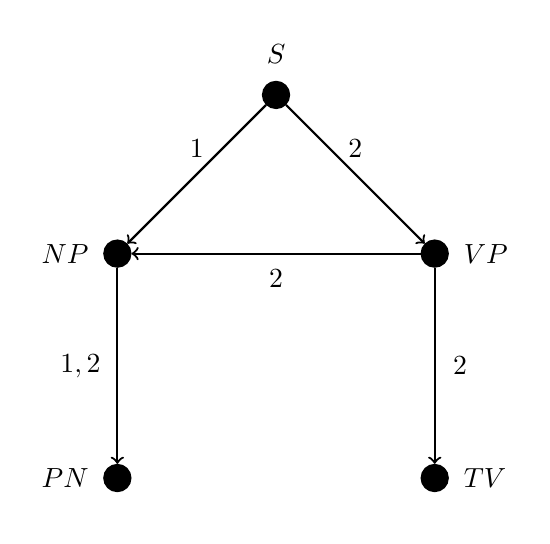
\begin{tikzpicture}[->,circle,draw,node distance=2.85cm,fill=black
                   ]

    \node[circle,label=90:$S$,draw,thick,fill=black](w0){$
    $};
    \node[circle,label=180:$NP$,below left of=w0,draw,thick,fill=black](w1){$
    $};
    \node[circle,label=0:$VP$,below right of=w0,draw,thick,fill=black](w2){$
    $};
    \node[circle,label=180:$PN$,below of=w1,draw,thick,fill=black](w3){$
    $};
    \node[circle,label=0:$TV$,below of=w2, draw,thick,fill=black](w4){$
    $};
    %\node[circle,label=90:$NP'$,below right of=w2, draw,thick,fill=black](w5){$
    %$};
    %\node[circle,label=0:$PN'$,below of=w5,draw,thick,fill=black](w6){$
    %$};
    \path[thick] (w0) edge [above] node {$1$} (w1)
    (w0) edge [above] node {$2$} (w2)
    (w1) edge [left] node {$1,2$} (w3)
    (w2) edge [right] node {$2$} (w4)
    (w2) edge [below] node {$2$} (w1);
    %(w5) edge [below] node {} (w6);

\end{tikzpicture} 
              \caption{Model for phase-structure}
                \label{example_linguistics}
    \end{subfigure}%
    \begin{subfigure}{.5\textwidth}
          \centering
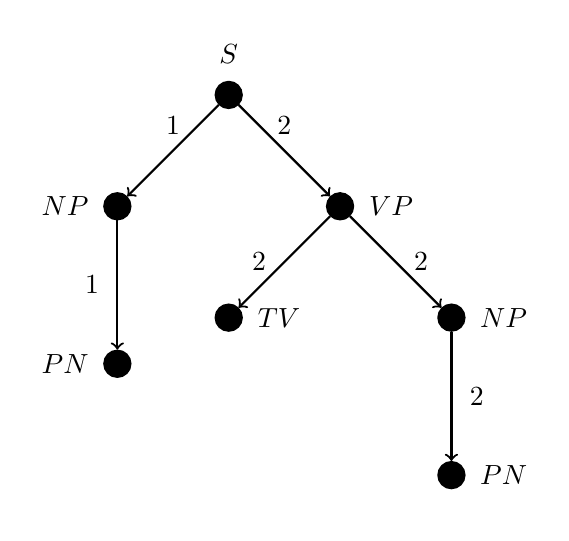
\begin{tikzpicture}[->,circle,draw,node distance=2cm,fill=black
                   ]

    \node[circle,label=90:$S$,draw,thick,fill=black](w0){$
    $};
    \node[circle,label=180:$NP$,below left of=w0,draw,thick,fill=black](w1){$
    $};
    \node[circle,label=0:$VP$,below right of=w0,draw,thick,fill=black](w2){$
    $};
    \node[circle,label=180:$PN$,below of=w1,draw,thick,fill=black](w3){$
    $};
    \node[circle,label=0:$TV$,below left of=w2, draw,thick,fill=black](w4){$
    $};
    \node[circle,label=0:$NP$,below right of=w2, draw,thick,fill=black](w5){$
    $};
    \node[circle,label=0:$PN$,below of=w5,draw,thick,fill=black](w6){$
    $};
    \path[thick] (w0) edge [above] node {$1$} (w1)
    (w0) edge [above] node {$2$} (w2)
    (w1) edge [left] node {$1$} (w3)
    (w2) edge [left] node {$2$} (w4)
    (w2) edge [right] node {$2$} (w5)
    (w5) edge [right] node {$2$} (w6);

\end{tikzpicture} 
              \caption{Tree-like model for phase-structure}
                \label{example_tree-like}
    \end{subfigure}
\end{figure}


 
    As trees play an important role in computer science, we will take this
    opportunity to define them. By a tree $\mathfrak{T}$ we mean a relational
    structure $(T, S)$ where $T$ is a set of nodes and $S$ is a binary relation
    over these nodes. $T$ contains a unique node $r_0 \in T$ (called the
    \emph{root}) such that all other nodes in $T$ are reachable from $r_0$, that
    is, for all $t \in T$, with $t \neq r_0$, we have $S^*r_0 t$, besides that,
    every element of $T$, distinct from $r_0$, has a unique $S$-predecessor, and
    the transitive and reflexive closure $S^+$ is acyclic, that is, for all $t
    \in T$, we have $\neg S^* t t$~\cite{areces2000tree}.

    A \emph{tree model} is a Kripke model $(W, \st_0, R, \pi)$, with $\Agents =
    \{1\}$, where $(W, R)$ is a tree and $\st_0$ is its root. A \emph{tree-like
    model} for \system{K}{n}{} is a model $(W, \st_0, R_1, \ldots, R_n, \pi)$,
    with $\Agents = \{1, \ldots, n\}$, such that $(W, \cup_{i \in \Agents} R_i)$
    is a tree, with $\st_0$ as the root.

    Let $\Model = (W, \st_0, R_1, \ldots, R_a, \pi)$ be a tree-like model for
    \system{K}{n}{}. We define the $depth: W \longrightarrow \Nat$ of a world
    $\st \in W$, as the length of the path from $\st_0$ to $\st$ through the
    union of the relations in \Model. We sometimes say $depth$ of \Model~to mean
    the longest path from the root to any world in $W$.

    The following theorems have been adapted from the ones presented
    in~\cite{areces2000tree}.

    \begin{theorem}%
        \label{theo:tl1}
        Let $\formula \in \wff$ be a formula and $\Model = (W, \st_0, R_1,
        \ldots, R_n, \pi)$ be a model. Then $\Model \models_L \formula$ if and only if
        there is a tree-like model $\Model'$ such that $\Model' \models_L \formula$.
        Moreover, $\Model'$ is finite and its $depth$ is bounded by
        $mdepth(\formula)$.
    \end{theorem}

    The proof of Theorem~\ref{theo:tl1} presented in~\cite{blackburn2002modal}
    constructs a tree-like model $\Model'$ as a \emph{generated submodel} of
    $\Model$, that is, it restricts the binary relations to consider only a
    subset of $W$. Then, using the satisfiability invariance of generated
    submodels, also proved in~\cite{blackburn2002modal}, which states that a
    formula is satisfiable in a model if, and only if, is satisfiable in its
    generated submodels, the proof becomes trivial.

    \begin{theorem}%
        \label{theo:tl2}
        Let $\formula, \formula' \in \wff$ and $\Model = (W, \st_0, R_1, \ldots,
        R_n, \pi)$ be a tree-like model such that $\Model \models_L \formula$. If
        $(\formula', \lambda', ml) \in \tau(\formula, 1, 0)$ and
        $\formula'$ is satisfied in $\Model$, then there is $\st \in W$, with
        $depth(w) = ml$, such that $\sat{\Model}{\st}{\formula'}$. Moreover,
        the subtree rooted at $w$ has height equals to $mdepth(\formula')$.
    \end{theorem}

    The proof of Theorem~\ref{theo:tl2} is by induction on the structure of the
    formula and shows that a subformula $\formula'$ of $\formula$ is satisfied
    at a node with distance $ml$ of the root of the tree-like model. As
    determining the satisfiability of a formula $\formula$ depends only on its
    subformulae $\formula'$, only the subtrees of height $mdepth(\formula')$
    starting at level $ml$ need to be checked. The bound on the height of the
    subtrees follows from Theorem~\ref{theo:tl1}~\cite{nalon2015modal}.
\end{example}

The \emph{local satisfiability problem} for \system{K}{n}{} corresponds to
determining the existence of a model in which a formula is locally satisfied,
while the \emph{global satisfiability problem} corresponds to determining the
existence of a model in which a formula is globally satisfied. These problems
are proven to be PSPACE-complete~\cite{Spaan:coml}, for local satisfiability,
and EXPTIME, for global satisfiability~\cite{Spaan:coml}.

The global satisfiability problem for a modal logic is equivalent to the local
satisfiability problem of the logic obtained by adding the universal modality,
$\nec{*}$, to the original modal language~\cite{goranko1992using}. Let
$\system{K}{n}{*}$ be the logic obtained by adding $\nec{*}$ to \system{K}{n}{}.
A model $\Model^*$ for \system{K}{n}{*} is the pair $(\Model, R_*)$, where
$\Model = (W, \st_0, R_1, \ldots, R_n, \pi)$ is a tree-like model for
\system{K}{n}{} and $R_* = W \times W$. The global satisfiability problem is
equivalent to the satisfiability problem in the following sense: a formula
$\nec{*} \formula$ is satisfied at the world $\st \in W$, in the model
$\Model^*$, written \sat{\Model^*}{\st}{\nec{*}\formula}, if, and only if, for
all $\st' \in W$, we have that \sat{\Model^*}{\st'}{\formula}. Therefore, let
$\formula \in \wff$ be a formula, we say that $\Model \models_G \formula$, if,
and only if, $\Model^* \models_L \nec{*} \formula$. 

\section{Proof Systems and Normal Forms}

%% LOGICAL CONSEQUENCE %%

The \emph{proof} of theorems, or the \emph{deduction} of consequences from
assumptions, in mathematics, typically is characterized by an argument that
follows from a (possibly empty) set of premises~\cite{kleene2002mathematical}.
These premises can be derived from a specific theory.

Formally, a proof is a finite object constructed according to a fixed set of
syntactic rules that refer only to the structure of formulae and not to their
intended meaning~\cite{fitting}. The set of syntactic rules that define proofs
are said to specify a \emph{proof system} or \emph{calculus}. These rules allow
the derivation of formulae from sets of formulae through strict symbol
manipulation~\cite{resolutionbased}. A proof system is \emph{sound} for a
particular logic if any formula that has a proof is a valid formula of the
logic, and it is \emph{complete} for a particular logic if any valid formula has
a proof~\cite{fitting}. Therefore, a sound and complete calculus allows us to
produce proofs that formulae are valid. 

A sound and complete calculus for \system{K}{n}{} finds a proof for a formula of
this logic if, and only if, this formula is valid. A proof for this
logic is defined in Section~\ref{sec:calc}.
%\begin{definition}%
%\label{def:kproof}
    %A \emph{\system{K}{n}{}-proof}, or a \emph{proof for \system{K}{n}{}}, is a
    %finite sequence of formulae, each of which is an axiom, or follows from one
    %or more earlier items in the sequence by applying a syntactic rule. The
    %axioms for \system{K}{n}{} are all instances of propositional tautologies
    %plus the axiom  \system{K}{}{}: $\nec{a}(\varphi \then \psi) \then (\nec{a}
    %\varphi \then \nec{a} \psi)$~\cite{blackburn2002modal}.
%\end{definition}
Propositional tautologies may contain modalities, for example, $\pos{}p \lor
\neg \pos{} q$ is a tautology. As tautologies are valid, they are a safe
starting point for modal reasoning. 

There are many kinds of proof systems. They can be loosely divide into two broad
categories: \emph{synthetic} and \emph{analytic}~\cite{fitting}. An analytic
proof system decomposes the formula being proved into simpler and simpler parts.
A synthetic proof system, on the other hand, builds its way up to the formula
being proved. Analytic proof systems tend to be easier to use, since the field
of play is sharply limited to the formula being proved~\cite{fitting}. 

The most common example of synthetic calculus is an \emph{axiomatic system}.
Certain formulae are taken as axioms. A proof starts with these axioms and,
using inference rules that produce new formulae, builds up a sequence that
finally ends with the formula being proved.

\emph{Tableau systems} are one of the more common analytic proof systems.  These
are \emph{refutational systems}, i.e., to prove a formula, we begin by negating
it, then analysing the entailment of doing so. If it is the case that the
consequences turn out to be impossible, we conclude that the original formula
has been proved~\cite{fitting}. There are many varieties of tableaux, and the
interesting thing about these systems is that, usually, proofs can be
represented by trees of formulae, instead of sequences as mentioned above.

Another way of categorizing proof systems involves the chaining in which the
rules are applied to form a line of reasoning. If the chaining starts from a set
of conditions and moves toward some (possibly remote) conclusion, the system is
called \emph{forward chaining}. If the conclusion is known, for instance, if it
is a goal to be achieved, but the path to this conclusion is unknown, then
reasoning backwards is called for, and the system is a \emph{backward
chaining}~\cite{feigenbaum1988rise}. Backward systems, in essence, start from
what is needed to be proved and moves towards the axioms.

Backward chaining is a standard technique in automated deduction, often taking
the form of a version of Robinson's \emph{resolution
rule}~\cite{harland2000forward}. Calculi based on this rule is often referred as
\emph{resolution-based systems}. The fundamental question is to determine
whether or not a given formula follows from a given set of formulae, and there
are various techniques which can be applied to guide the search for a proof.
Resolution systems for propositional logic perform this search by thoroughly
applying a single rule, with the goal of obtaining a contradiction, since it is
also a refutational system. This one rule is showed in
Chapter~\ref{3_Resolution}, where we briefly introduce the resolution system.

In the literature, there are several kinds of proof systems proposed for
\system{K}{n}{}. The one we use in this work is based in resolution, it was
proposed by~\cite{nalon2015modal} and it is also presented in
Chapter~\ref{3_Resolution}. The calculus used is proved to be sound and complete
for \system{K}{n}{} in~\cite{nalon2015modal}, it was developed with regard to
computer implementations and it uses formulae translated into a special
\emph{normal form}.

A normal form is an elegant representation of an equivalence class and the
equivalence relation in question may determine what kind of normal form is
used~\cite{normalformtheory}. The relation considered in proof systems for logic
languages relates two formulae if whenever one is satisfiable, the other one
also is. Therefore, the transformation rules defined for a specific normal form
used in a proof system for a logic must preserve satisfiability, that is, the
formula obtained by applying a transformation rule is satisfiable if, and only
if, the original one also is. 

Formulae translated into a normal form have a specific, normalized structure,
possibly resulting in less operators to handle with, which may implicate into a
smaller number of rules for a proof system. Hence, a calculus that is planned to
be implemented in a computer may take great advantage of normal forms, since the
smaller number of rules reduces the chances of implementation errors, for
example. 

The normal form used in this work is a layered normal form called Separated
Normal Form with Modal Levels, originally proposed
in~\cite{journals/jal/NalonD07}. This normal form is introduced in
Chapter~\ref{3_Resolution}, as well as the translation rules for formulae in
\system{K}{n}{}. The proof that this translation preserves satisfiability can be
found in~\cite{journals/jal/NalonD07}.
